 \section{Unidad 1}
           \subsection{L1 Conocimiento empírico}

          \ejemplosboxed[6]{Señala si son \textit{verdaderas} o \textit{falsas} las siguientes frases:
         
          \begin{multicols}{2}
               \begin{parts}
                    \part El conocimiento empírico se obtiene a través del método científico y la experimentación controlada.

                    \begin{oneparchoices}
                         \choice Verdadero \CorrectChoice Falso
                    \end{oneparchoices}

                    \part El conocimiento empírico es subjetivo y puede variar entre diferentes individuos.

                    \begin{oneparchoices}
                         \CorrectChoice Verdadero \choice Falso
                    \end{oneparchoices}

                    \part El conocimiento empírico usa el razonamiento lógico.

                    \begin{oneparchoices}
                         \choice Verdadero \CorrectChoice Falso
                    \end{oneparchoices}

                    \part El conocimiento empírico puede estar sujeto a preferencias personales y limitaciones sensoriales.

                    \begin{oneparchoices}
                         \CorrectChoice Verdadero \choice Falso
                    \end{oneparchoices}

                    \part El conocimiento empírico siempre es preciso y objetivo.

                    \begin{oneparchoices}
                         \choice Verdadero \CorrectChoice Falso
                    \end{oneparchoices}

                    \part La base del conocimiento empírico se basa en las experiencias del individuo.

                    \begin{oneparchoices}
                         \CorrectChoice Verdadero \choice Falso
                    \end{oneparchoices}

               \end{parts}
          \end{multicols}
     }

 \questionboxed[5]{Elige la(s) respuesta(s). Puede existir más de una respuesta correcta.
         
            \begin{multicols}{2}
                 \begin{parts}
                      \part Son características del conocimiento empírico:
  
                      \begin{oneparcheckboxes}
                           \CorrectChoice subjetivo
                           \choice objetivo
                           \choice sistemático
                           \CorrectChoice limitado a la percepción
                           \CorrectChoice práctico
                           \choice basado en teorías
                      \end{oneparcheckboxes}

    \part  Son ejemplos de conocimiento empírico:
  
                      \begin{checkboxes}
                           \CorrectChoice observar el color y tamaño de las nubes para predecir el clima.
                           \choice la teoría de que las especies cambian con el tiempo a través de procesos de selección natural y mutación.
                           \CorrectChoice saber que el agua caliente puede aliviar el dolor muscular.
                           \choice saber que el peso es una fuerza y por lo tanto una cantidad vectorial.
                           \choice dar una explicación sobre los cambios de estado del agua, relacionados con los cambios en su estructura interna.
                      \end{checkboxes}
  
                      \part Que el conocimiento sea asistemático significa que:
  
                      \begin{checkboxes}
                           \choice se ajusta a un sistema ordenado y con procedimientos.
                           \choice sigue un método organizado en el que se plantean pasos a seguir.
                           \choice depende de la percepción personal que afirma el conocimiento.
                           \CorrectChoice se obtiene de forma casual y sin una metodología organizada.
                      \end{checkboxes}

                      \columnbreak%

                      \part  El conocimiento empírico se basa en:
  
                      \begin{checkboxes}
                           \choice causas e hipótesis.
                           \CorrectChoice experiencias personales.
                           \choice aprender conocimientos en la escuela.
                           \CorrectChoice observar que una acción necesariamente provoca otra.
                           \choice el planteamiento de una teoría y la experimentación en el laboratorio.
                      \end{checkboxes}

                      \part Es una forma  de aprender mediante la observación de tu entorno, tus sentidos y las experiencias en tu vida cotidiana.
  
                      \begin{checkboxes}
                           \choice Aprendizaje experimental
                           \CorrectChoice Conocimiento empírico
                           \choice Educación continua
                           \choice Conocimiento científico
                      \end{checkboxes}

                      \part Si el conocimiento se obtiene a partir de los sentidos y tiene alguna limitación a los mismos, significa que es:
  
                      \begin{checkboxes}
                           \choice enfocado en el aprendizaje sistemático.
                           \CorrectChoice limitado a la percepción.
                           \choice basado en procedimientos y observación.
                           \choice orientado por la experimentación.
                      \end{checkboxes}
                 \end{parts}
            \end{multicols}
       }

            \questionboxed[3]{Elige la respuesta correcta.
        
     \begin{multicols}{2}
               \begin{parts}
                       \part Los conocimientos tradicionales son:

                    \begin{choices}
                         \CorrectChoice transmitidos de generación en generación en una cultura y que les da identidad
                         \choice las técnicas y procedimientos para producir arte
                         \choice consideraciones de lo justo o injusto para la convivencia en una comunidad.
                         \choice útiles para resolver problemas prácticos en la vida cotidiana.
                    \end{choices}

 \part  Los conocimientos políticos se refieren a \dots

                    \begin{choices}
                         \choice métodos para producir o transformar la naturaleza
                         \choice lo que la sociedad considera bueno o malo y necesario para la convivencia.
                         \choice los que se utilizan para obtener un bien material o resolver un problema real.
                         \CorrectChoice la organización y forma de gobierno de la sociedad.
                    \end{choices}

\columnbreak%

                    \part  Los conocimientos \rule{50pt}{0.2pt} son las técnicas y procedimientos desarrollados para producir escultura, pintura o música.

                   % \begin{multicols}{2}
                    \begin{choices}
                         \choice morales
                         \CorrectChoice artísticos
                         \choice técnicos
                         \choice prácticos
                    \end{choices}
              % \end{multicols}

                
                    \part Los conocimientos \rule{50pt}{0.2pt} son los que se usan para resolver un problema u obtener un bien material.

                    %\begin{multicols}{2}
                    \begin{choices}
                         \choice morales
                         \choice técnicos
                         \choice artísticos
                         \CorrectChoice prácticos
                    \end{choices}
              % \end{multicols}

                    \part  Son tipos de conocimiento empírico

                  % \begin{multicols}{2}
                    \begin{choices}
                         \CorrectChoice artísticos.
                         \choice teóricos.
                         \CorrectChoice tradicionales.
                         \choice sistemáticos.
                         \choice científicos
                     \end{choices}
               % \end{multicols}

                    

               \end{parts}
          \end{multicols}
     }

 % \addcontentsline{toc}{section}{L2 El conocimiento científico}
            \subsection{L2 El conocimiento científico}

      \ejemplosboxed[9]{Ordena los pasos del método científico.

          \begin{parts}
               \part \fillin[5][0.2in] Análisis de resultados
               \part \fillin[4][0.2in] Experimentación
               \part \fillin[7][0.2in] Comunicación de resultados
               \part \fillin[9][0.2in] Teoría científica
               \part \fillin[1][0.2in] Observación
               \part \fillin[8][0.2in] Ley científica
               \part \fillin[2][0.2in] Planteamiento del problema
               \part \fillin[6][0.2in] Verificación de la hipótesis
               \part \fillin[3][0.2in] Hipótesis
          \end{parts}
     }

       \questionboxed[3]{Elige la respuesta correcta
       \begin{multicols}{2}
            \begin{parts}
                 \part Indica con claridad el problema que se quiere resolver. Delimita y especifica el objeto de su investigación.

                 \begin{choices}
                      \choice Experimentación
                      \CorrectChoice Planteamiento del problema
                      \choice Ley científica
                      \choice Comunicación de resultados
                 \end{choices}

                 \part Se trata de demostrar si la hipótesis es o no correcta mediante un experimento controlado.

                 \begin{choices}
                      \choice Hipótesis
                      \choice Observación
                      \choice Teoría científica
                      \CorrectChoice Experimentación
                 \end{choices}

                 \part Indica la regularidad que existe en un fenómeno, entre sus causas y sus efectos, normalmente se expresa de manera matemática.

                 \begin{choices}
                      \choice Hipótesis
                      \CorrectChoice Ley científica
                      \choice Teoría científica
                      \choice Experimentación
                 \end{choices}

                 \part Si no se comprueba la hipótesis, se plantea una nueva, considerando los datos y la información obtenida en el experimento.

                 \begin{choices}
                      \CorrectChoice Verificación de la hipótesis
                      \choice Análisis de resultados
                      \choice Teoría científica
                      \choice Comunicación de resultados
                 \end{choices}

                 \columnbreak

                 \part El científico observa la realidad que le rodea, aísla el fenómeno que le interesa e identifica las variables que intervienen.

                 \begin{choices}
                      \choice Hipótesis
                      \CorrectChoice Observación
                      \choice Teoría científica
                      \choice Verificación de la hipótesis
                 \end{choices}

                 \part Propuesta de una posible explicación del fenómeno.

                 \begin{choices}
                      \CorrectChoice Hipótesis
                      \choice Observación
                      \choice Teoría científica
                      \choice Experimentación
                 \end{choices}

                 \part La hipótesis se confirma o se rechaza analizando los datos y la información obtenida en los experimentos.

                 \begin{choices}
                      \choice Ley científica
                      \choice Observación
                      \CorrectChoice Análisis de resultados
                      \choice Experimentación
                 \end{choices}

                 \part El científico comparte los resultados de su investigación a la comunidad científica mediante tesis, artículos científicos o congresos.

                 \begin{choices}
                      \choice Ley científica
                      \choice Análisis de resultados
                      \choice Teoría científica
                      \CorrectChoice Comunicación de resultados
                 \end{choices}

                 \part Explicación de un fenómeno a partir de leyes científicas.

                 \begin{choices}
                      \CorrectChoice Teoría científica
                      \choice Ley científica
                      \choice Análisis de resultados
                      \choice Comunicación de resultados
                 \end{choices}
            \end{parts}
       \end{multicols}
  }

  \questionboxed[3]{Analiza el texto y selecciona las palabras para completar las afirmaciones:

 \begin{center}
            \wordpill{Biología}    
              \wordpill{metódica} 
              \wordpill{predictiva}  
               \wordpill{demostrable}
               \wordpill{Física}  
            \wordpill{Matemáticas}  
          \end{center}
          \vspace*{1em}

\begin{parts}
    \part La ciencia es el tipo de conocimiento basado en la observación, el razonamiento, la experimentación y la comprobación. Sus características son: Objetiva porque se basa en un objeto de estudio, \fillin[demostrable] porque es comprobable por experiencia directa, \fillin[metódica] porque sigue un procedimiento ordenado y \fillin[predictiva] porque es aplicable a fenómenos similares.
    
    \part La ciencia se divide en:
    \begin{itemize}
        \item \textbf{Ciencia formal}, su objeto de estudio son las ideas, conceptos que existen en el razonamiento humano, como la Lógica, \fillin[Matemáticas] y Ciencias de la computación.
        \item \textbf{Ciencia fáctica}, su objeto de estudio son las cosas materiales, reales y concretas, como la \fillin[Física], Química y \fillin[Biología].
    \end{itemize}
\end{parts}
}

% \questionboxed[5]{Encierra el par de conceptos que completa correctamente cada afirmación.

% \begin{parts}
%     \part En la antigua Grecia se desarrolló por primera vez una forma \_\_\_\_\_\_\_\_\_ de pensar acerca de los fenómenos naturales, alejada de las creencias y \_\_\_\_\_\_\_\_\_.
%     \begin{choices}
%         \choice ordenada / las ambigüedades
%         \choice organizada / las falacias
%         \choice racional / los dogmas
%     \end{choices}

%     \part Newton pensaba que la luz estaba formada por \_\_\_\_\_\_\_\_\_ en movimiento. Así explicaba el fenómeno de \_\_\_\_\_\_\_\_\_ con el cambio en dirección y rapidez de la luz al pasar de un medio a otro.
%     \begin{choices}
%         \choice partículas / refracción
%         \choice ondas / reflexión
%         \choice fotones / polarización
%     \end{choices}

%     \part El modelo cinético corpuscular de la materia propuesto por \_\_\_\_\_\_\_\_\_ suponía que la materia estaba formada por \_\_\_\_\_\_\_\_\_.
%     \begin{choices}
%         \choice James C. Maxwell / grandes estructuras moleculares
%         \choice Daniel Bernoulli / pequeñas esferas sólidas
%         \choice Ludwig Boltzmann / átomos idénticos
%     \end{choices}

%     \part Maxwell y Boltzmann propusieron que un gas estaba formado por \_\_\_\_\_\_\_\_\_ sólidas en movimiento continuo que colisionaban \_\_\_\_\_\_\_\_\_ del recipiente que lo contenía.
%     \begin{choices}
%         \choice pequeñas esferas / entre sí y con las paredes
%         \choice estructuras moleculares / sólo con las paredes
%     \end{choices}

%     \part La teoría corpuscular de Newton fue bien recibida, pero no explicaba por qué si la luz estaba formada por \_\_\_\_\_\_\_\_\_, la masa de las fuentes de luz no \_\_\_\_\_\_\_\_\_ al emitirla.
%     \begin{choices}
%         \choice corpúsculos / disminuye
%         \choice ondas / aumenta
%         \choice electrones / permanece constante
%     \end{choices}
    
%     \part En 1827, el botánico inglés Robert Brown observó que los granos de polen \_\_\_\_\_\_\_\_\_, homogéneamente distribuidos, se mueven \_\_\_\_\_\_\_\_\_. A esto se le llamó ``movimiento browniano''.
%     \begin{choices}
%         \choice en agua hirviendo / muy deprisa
%         \choice inmersos en un líquido / aleatoriamente en todas direcciones
%     \end{choices}

%     \part Albert Einstein analizó el fenómeno de movimiento browniano y dedujo que el movimiento \_\_\_\_\_\_\_\_\_ del polen en suspensión se debe a \_\_\_\_\_\_\_\_\_ de las moléculas con las partículas de polen.
%     \begin{choices}
%         \choice oscilatorio / las cohesiones
%         \choice azaroso / las colisiones
%         \choice veloz / los enlaces
%     \end{choices}
% \end{parts}
% }
    
\subsection{L3 Física y sociedad}

 \ejemplosboxed[9]{Coloca los conceptos en el lugar que les corresponda en la imagen.

          \begin{center}
               \wordpill{Mecánica estadiática}
               \wordpill{Estudia los átomos y su constitución}
               \wordpill{Relatividad}
               \wordpill{Fuerza}
               \wordpill{Acústica}
               \wordpill{Describe el movimiento de los objetos}
               \wordpill{Física clásica}
               \wordpill{Física moderna}
               \wordpill{Calor y temperatura}
               \vspace*{1em}
               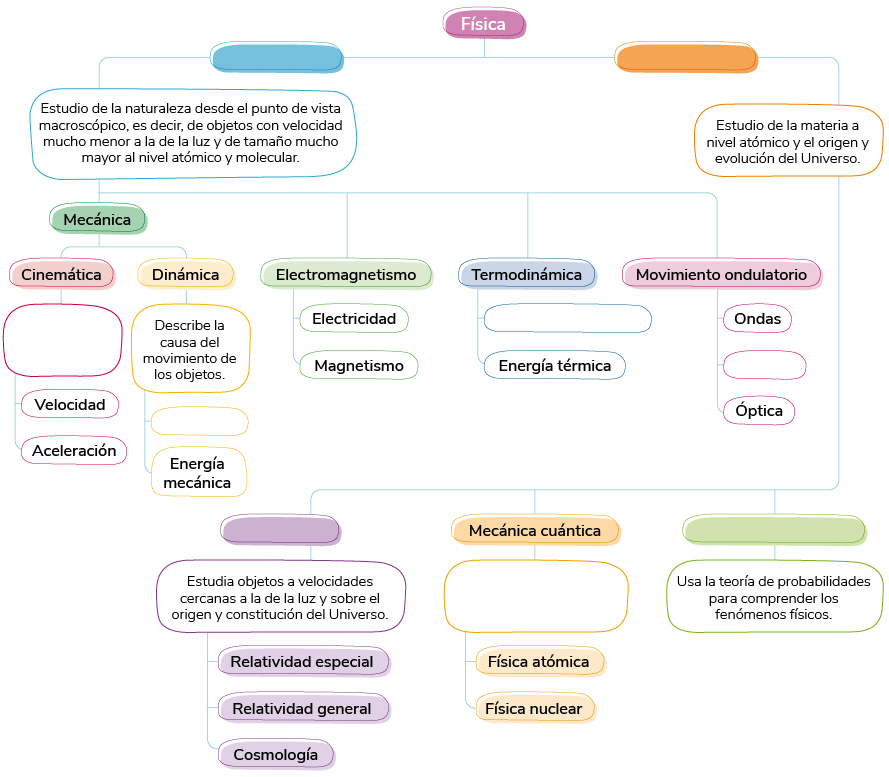
\includegraphics[width=.85\textwidth]{../images/SIM_FI2_SB_U1_P28_IMG01.jpg}
          \end{center}
     }

 \questionboxed[11]{Coloca las palabras que completan los párrafos.
        
\begin{center}
               \wordpill{empírico}
               \wordpill{argumentación}
               \wordpill{científico}
               \wordpill{asistemático}
               \wordpill{religioso}
               \wordpill{ciencia}
               \wordpill{sistematizado}
               \wordpill{Galileo Galilei}
               \wordpill{razón}
               \wordpill{método científico}
               \wordpill{los cráteres de la Luna}
          \end{center}
          \vspace*{1em}
          \begin{parts}
               \part Antes del siglo XVI en las academias y universidades de Europa el conocimiento se sustentaba en la filosofía, y consistía en la reflexión basada en la \fillin[argumentación][1in] y la \fillin[razón][1in] lógica heredadas de la cultura griega y romana.
               \part En los talleres se transmitía y enseñaba el trabajo de los artesanos mediante el conocimiento \fillin[empírico][1in] y la práctica.
               \part Por su parte, la sociedad se organizaba y convivía con base en el conocimiento \fillin[religioso][1in].
               \part Estas formas de conocimiento han perdurado hasta nuestros días, pero en el siglo XVI inició el desarrollo de una nueva forma de conocer la realidad: el conocimiento \fillin[científico][1in].
               \part \fillin[Galileo Galilei][1in] desarrolló, en el siglo XVI, un telescopio a partir de un catalejo, para observar los cuerpos celestes. Este científico observó con su telescopio \fillin[los cráteres de la Luna][2in] por primera vez.
               \part Una de las aportaciones más importante de Galileo Galilei fueron los experimentos cuantificados, pues relacionó los fenómenos físicos con las matemáticas, lo cual dio origen al \fillin[método científico][1.5in].
               \part Que el conocimiento sea \fillin[asistemático][1in] significa que se obtiene de forma casual y sin una metodología organizada.
               \part El objetivo de la \fillin[ciencia][1in] es explicar los fenómenos naturales a partir de la observación, la experimentación, el razonamiento y la comprobación.
               \part A diferencia del conocimiento empírico, el conocimiento científico es \fillin[sistematizado][1in], lo que significa que sigue un método.
          \end{parts}
     }


     \questionboxed[4]{Señala si los siguientes procesos son \textit{físicos} o \textit{químicos}.
 
     \begin{multicols}{2}
          \begin{parts}
               \part Romper una hoja de papel.

               \begin{oneparchoices}
                    \CorrectChoice Físico \choice Químico
               \end{oneparchoices}

               \part Digerir y absorber los alimentos.

               \begin{oneparchoices}
                    \choice Físico \CorrectChoice Químico
               \end{oneparchoices}

               \part Derretir una vela.

               \begin{oneparchoices}
                    \CorrectChoice Físico \choice Químico
               \end{oneparchoices}

               \part Encender fuegos artificiales.

               \begin{oneparchoices}
                    \choice Físico \CorrectChoice Químico
               \end{oneparchoices}

               \part Hornear un pastel de vainilla.

               \begin{oneparchoices}
                    \choice Físico \CorrectChoice Químico
               \end{oneparchoices}

               \part Apretar una lata de aluminio.

               \begin{oneparchoices}
                    \CorrectChoice Físico \choice Químico
               \end{oneparchoices}

               \part Derretir un cubo de hielo.

               \begin{oneparchoices}
                    \CorrectChoice Físico \choice Químico
               \end{oneparchoices}

               \part Cocinar un huevo estrellado.

               \begin{oneparchoices}
                    \choice Físico \CorrectChoice Químico
               \end{oneparchoices}
          \end{parts}
     \end{multicols}
}

\questionboxed[5]{Clasifica las siguientes ramas escribiendo \textbf{C} si pertenecen a la Física Clásica o \textbf{M} si pertenecen a la Física Moderna:

\begin{multicols}{3}

     \begin{parts}
    \part \fillin[C][1cm] Mecánica
    \part \fillin[C][1cm] Electromagnetismo
    \part \fillin[C][1cm] Termodinámica
    \part \fillin[M][1cm] Relatividad
    \part \fillin[M][1cm] Mecánica cuántica
\end{parts}
\end{multicols}
}
   
         \questionboxed[5]{Completa las siguientes afirmaciones con la palabra correcta:

    \begin{center}
               \wordpill{espacio}
               \wordpill{físicos}
               \wordpill{científico}
               \wordpill{ciencia}
               \wordpill{partículas}
               \wordpill{átomos}
               \wordpill{una fuerza}
               \wordpill{tiempo}
               \wordpill{la materia}
               \wordpill{naturaleza}
          \end{center}
          \vspace*{1em}

    \begin{parts}
    \part La Física es una \fillin[ciencia] que utiliza el método \fillin[científico] para obtener sus conocimientos.
    \part La Física estudia la \fillin[naturaleza] y los fenómenos que ocurren en ella, incluso su origen y su posible final.
    \part También estudia el Universo y sus componentes fundamentales, como los \fillin[átomos] y las \fillin[partículas] que los forman.
    \part Los cambios que experimentan los objetos y que no alteran su composición se denominan cambios \fillin[físicos].
    \part La Física estudia la relación entre \fillin[la materia] y la energía, la interacción entre objetos, el cambio producido por \fillin[una fuerza] y dónde y cuándo tienen lugar los fenómenos, es decir, el \fillin[espacio] y el \fillin[tiempo].
\end{parts}

    }

    \questionboxed[3]{Relaciona los siguientes conceptos con la rama de la Física que les corresponde. Escribe la letra en el paréntesis.

    \begin{multicols}{2}
    \begin{enumerate}
        \item[A)] Física clásica
        \item[B)] Física moderna
        \item[C)] Cinemática
        \item[D)] Dinámica
        \item[E)] Termodinámica
        \item[F)] Acústica
    \end{enumerate}
    \columnbreak
    \begin{parts}
          \part (\fillin[F][1cm]) Rama del movimiento ondulatorio que estudia el sonido.
          \part (\fillin[C][1cm]) Describe el movimiento de los objetos.
          \part (\fillin[B][1cm]) Estudia fenómenos a nivel atómico y el origen del Universo.
          \part (\fillin[A][1cm]) Estudia fenómenos a velocidades mucho menores a la de la luz.
          \part (\fillin[E][1cm]) Estudia el calor y la temperatura.
          \part (\fillin[D][1cm]) Estudia la causa del movimiento de los objetos (fuerza).
    \end{parts}
\end{multicols}
    }

\questionboxed[3]{Determina a qué rama de la física corresponde cada uno de los siguientes escenarios o sistemas de estudio:

\begin{parts}
    \part Un termómetro midiendo altas temperaturas expuesto al sol:

    \begin{oneparchoices}
        \CorrectChoice Termodinámica 
        \choice Óptica 
        \choice Acústica 
        \choice Cosmología
    \end{oneparchoices}
    
    \part Antenas de telecomunicaciones emitiendo señales:

    \begin{oneparchoices}
        \choice Dinámica 
        \CorrectChoice Electromagnetismo 
        \choice Cinemática 
        \choice Óptica
    \end{oneparchoices}
    
%     \part La observación de una nebulosa en el espacio profundo:

%     \begin{oneparchoices}
%         \choice Termodinámica 
%         \choice Dinámica 
%         \CorrectChoice Cosmología 
%         \choice Acústica
%     \end{oneparchoices}
    
    \part Uso de un microscopio en un laboratorio:

    \begin{oneparchoices}
        \choice Electromagnetismo 
        \choice Cosmología
         \choice Acústica 
        \CorrectChoice Óptica
    \end{oneparchoices}
    
    \part Automóviles de Fórmula 1 compitiendo en una pista (estudio de su movimiento):

    \begin{oneparchoices}
        \choice Termodinámica 
        \CorrectChoice Cinemática 
        \choice Óptica 
        \choice Electromagnetismo
    \end{oneparchoices}
    
    \part Una orquesta sinfónica en pleno concierto:

    \begin{oneparchoices}
        \choice Dinámica 
        \CorrectChoice Acústica 
        \choice Cosmología
         \choice Cinemática
    \end{oneparchoices}
    
    \part Una persona empujando un automóvil descompuesto (estudio de las fuerzas):

    \begin{oneparchoices}
        \choice Termodinámica 
        \choice Acústica 
        \choice Óptica 
        \CorrectChoice Dinámica
    \end{oneparchoices}
\end{parts}
}

      \subsection{L4 Mediciones}

      \ejemplosboxed[7]{Elige la(s) respuesta(s). Puede existir más de una respuesta correcta.

      \begin{multicols}{2}
           \begin{parts}
                \part Son algunas unidades de medida que se utilizaban en la antigüedad:

                \begin{oneparcheckboxes}
                     \choice Libra
                     \CorrectChoice Pie
                     \choice Yarda
                     \CorrectChoice Codo
                \end{oneparcheckboxes}

                \part Los mexicas tenían unidades de medida de longitud como el \rule{50pt}{0.2pt} que era un palo de madera que medía aproximadamente dos metros y medio.

                \begin{oneparcheckboxes}
                     \choice Testal
                     \CorrectChoice Tlalcuahuitl\\
                     \choice Cenequeztzalli
                     \choice Omitl
                \end{oneparcheckboxes}

                \columnbreak%

                \part Son medidas de longitud usadas en México en la época colonial:

                \begin{oneparcheckboxes}
                     \CorrectChoice Legua
                     \choice Testal
                     \CorrectChoice Vara
                     \choice Arroba
                \end{oneparcheckboxes}


                \part La \rule{50pt}{0.2pt} es la medida de la palma de la mano extendida.

                \begin{oneparcheckboxes}
                     \choice Legua
                     \choice Vara
                     \CorrectChoice Cuarta
                     \choice yYarda
                \end{oneparcheckboxes}

                \part La arroba fue una unidad de medida de \rule{50pt}{0.2pt} en la época colonial.

                \begin{oneparcheckboxes}
                     \choice Tiempo
                     \choice Distancia
                     \CorrectChoice Peso
                     \choice Masa
                \end{oneparcheckboxes}

           \end{parts}
      \end{multicols}
 }

 \questionboxed[5]{Utiliza las siguientes palabras para completar las afirmaciones: \textit{comparar, cuantificar, medición, precisión, referencia}.

  \begin{center}
              \wordpill{referencia}
               \wordpill{cuantificar} 
              \wordpill{precisión}  
                \wordpill{comparar}
               \wordpill{medición}  
          \end{center}
          \vspace*{1em}
 \begin{parts}
    \part Medir significa \fillin[comparar] dos cantidades con un instrumento de \fillin[medición].
    \part Una unidad de medida es una \fillin[referencia] que permite estimar una propiedad que se puede \fillin[cuantificar] con cierta exactitud.
    \part La forma de medir en la antigüedad era muy diferente a como lo hacemos en la actualidad, la principal diferencia es la \fillin[precisión] del instrumento con el que se mide.
\end{parts}
 }

% \questionboxed[5]{Marca la(s) respuesta(s) correcta(s) para cada enunciado (puede haber más de una):
% \begin{parts}
%     \part Son algunas unidades de medida que se utilizaban en la antigüedad:
%     \begin{checkboxes}
%         \choice Libra
%         \CorrectChoice Pie
%         \choice Yarda
%         \CorrectChoice Codo
%         \choice Metro
%     \end{checkboxes}
    
%     \part Los mexicas tenían unidades de medida de longitud, como el \rule{2cm}{0.15mm} que era un palo de madera que medía aproximadamente dos metros y medio.
%     \begin{checkboxes}
%         \choice testal
%         \choice cenequeztzalli
%         \choice omitl
%         \CorrectChoice tlalcuahuitl
%     \end{checkboxes}
    
%     \part Son medidas de longitud usadas en México en la época colonial:
%     \begin{checkboxes}
%         \CorrectChoice Legua
%         \choice Testal
%         \CorrectChoice Vara
%         \choice Arroba
%     \end{checkboxes}
    
%     \part La \rule{2cm}{0.15mm} es la medida de la palma de la mano extendida.
%     \begin{checkboxes}
%         \choice legua
%         \choice vara
%         \CorrectChoice cuarta
%         \choice yarda
%     \end{checkboxes}
    
%     \part La arroba fue una unidad de medida de \rule{2cm}{0.15mm} en la época colonial.
%     \begin{checkboxes}
%         \choice moral
%         \CorrectChoice peso
%         \choice técnico
%         \choice práctico
%     \end{checkboxes}
% \end{parts}
% }

      \subsection{L5 Unidades fundamentales y derivadas de medida}

      \ejemplosboxed[6]{Señala si son \textit{verdaderas} o \textit{falsas} las siguientes frases:

          \begin{multicols}{2}
               \begin{parts}\footnotesize%
                    \part En el SI la unidad para medir la capacidad es el metro cúbico.

                    \begin{oneparchoices}
                         \choice Verdadero \CorrectChoice Falso
                    \end{oneparchoices}
                    \part En el SI la unidad para medir el volumen es el metro cúbico.

                    \begin{oneparchoices}
                         \CorrectChoice Verdadero \choice Falso
                    \end{oneparchoices}
                    \part Cuando comparamos dos cuerpos con distinta composición química, el de mayor masa debe tener necesariamente mayor número de partículas.

                    \begin{oneparchoices}
                         \choice Verdadero \CorrectChoice Falso
                    \end{oneparchoices}
                    \part En modelo cinético de partículas se considera que la materia está constituida por partículas sin masa.

                    \begin{oneparchoices}
                         \choice Verdadero \CorrectChoice Falso
                    \end{oneparchoices}
                    \part Según el modelo cinético, la densidad indica la concentración de partículas de una sustancia en cierto volumen.

                    \begin{oneparchoices}
                         \CorrectChoice Verdadero \choice Falso
                    \end{oneparchoices}
                    \part El aire y el helio tienen una compresibilidad diferente.

                    \begin{oneparchoices}
                         \CorrectChoice Verdadero \choice Falso
                    \end{oneparchoices}
               \end{parts}
          \end{multicols}
     }

     \ejemplosboxed[7]{Relaciona las magnitudes físicas fundamentales con su unidad de medida en el Sistema Internacional.

          \begin{multicols}{2}
               \begin{parts}\raggedleft
                    \part Longitud              \fillin[E][0.2in]
                    \part Temperatura           \fillin[B][0.2in]
                    \part Cantidad de sustancia \fillin[G][0.2in]
                    \part Corriente eléctrica   \fillin[D][0.2in]
                    \part Intensidad luminosa   \fillin[F][0.2in]
                    \part Tiempo                \fillin[A][0.2in]
                    \part Masa                  \fillin[C][0.2in]
               \end{parts}

               \columnbreak

               \begin{choices}
                    \choice Segundo
                    \choice Kelvin
                    \choice Kilogramo
                    \choice ampere
                    \choice Metro
                    \choice candela
                    \choice mol
               \end{choices}
          \end{multicols}
     }

\questionboxed[4]{Clasifica las siguientes unidades de medida históricas según la magnitud física que evaluaban (Capacidad, Longitud o Peso):

\begin{multicols}{3}
\begin{itemize}
    \item Barril: \fillin[Capacidad][3cm]
    \item Codo: \fillin[Longitud][3cm]
    \item Arroba: \fillin[Peso][3cm]
    \item Pinta: \fillin[Capacidad][3cm]
    \item Vara: \fillin[Longitud][3cm]
    \item Legua: \fillin[Longitud][3cm]
    \item Botija: \fillin[Capacidad][3cm]
    \item Testal: \fillin[Peso][3cm]
\end{itemize}
\end{multicols}
}



\questionboxed[5]{Relaciona las magnitudes físicas fundamentales con su unidad de medida en el Sistema Internacional, escribiendo la letra correspondiente en el paréntesis.

\vspace{0.3cm}
\begin{minipage}[t]{0.45\textwidth}
    \begin{itemize}
        \item[(\quad)] Longitud
        \item[(\quad)] Tiempo
        \item[(\quad)] Masa
        \item[(\quad)] Temperatura
        \item[(\quad)] Corriente eléctrica
        \item[(\quad)] Intensidad luminosa
        \item[(\quad)] Cantidad de sustancia
    \end{itemize}
\end{minipage}
\hfill
\begin{minipage}[t]{0.45\textwidth}
    \begin{itemize}
        \item[E.] Candela
        \item[B.] Ampere
        \item[D.] Metro
        \item[G.] Kelvin
        \item[C.] Kilogramo
        \item[A.] Segundo
        \item[F.] Mol
    \end{itemize}
\end{minipage}
}

     %  \addcontentsline{toc}{section}{L6 Múltiplos y submúltiplos}
\subsection{L6 Múltiplos y submúltiplos}

\ejemplosboxed[8]{Señala si son \textit{verdaderas} o \textit{falsas} las siguientes frases:

\begin{multicols}{2}
     \begin{parts}
          \part Las unidades derivadas resultan de combinar dos o más unidades fundamentales.

          \begin{oneparchoices}
               \choice Verdadero \CorrectChoice Falso
          \end{oneparchoices}

          % \part Los grados Celsius son una unidad fundamental.

          % \begin{oneparchoices}
          %      \CorrectChoice Verdadero \choice Falso
          % \end{oneparchoices}

          \part Para medir la velocidad se combinan unidades de distancia y de tiempo.

          \begin{oneparchoices}
               \choice Verdadero \CorrectChoice Falso
          \end{oneparchoices}

          \part El área combina tres veces las unidades de longitud, como los metros cúbicos.

          \begin{oneparchoices}
               \CorrectChoice Verdadero \choice Falso
          \end{oneparchoices}

          \part Los newtons son una unidad derivada.

          \begin{oneparchoices}
               \CorrectChoice Verdadero \choice Falso
          \end{oneparchoices}

          \columnbreak

          \part El milímetro es un múltiplo del metro

          \begin{oneparchoices}
               \CorrectChoice Verdadero \choice Falso
          \end{oneparchoices}

          \part El kilogramo es un múltiplo del gramo.

          \begin{oneparchoices}
               \CorrectChoice Verdadero \choice Falso
          \end{oneparchoices}

          \part Los múltiplos del segundo se utilizan para medir tiempos muy pequeños.

          \begin{oneparchoices}
               \CorrectChoice Verdadero \choice Falso
          \end{oneparchoices}

          \part Los múltiplos del metro se utilizan para medir distancias y longitudes muy grandes.

          \begin{oneparchoices}
               \CorrectChoice Verdadero \choice Falso
          \end{oneparchoices}
     \end{parts}
\end{multicols}

}

\questionboxed[5]{Relaciona el prefijo de las unidades con su escala de multiplicación o división correspondiente.

\begin{multicols}{2}

     \begin{choices}
    \choice \textbf{giga} \fillin{a}
    \choice \textbf{nano} \fillin{d}
    \choice \textbf{deci} \fillin{b}
    \choice \textbf{kilo} \fillin{e}
    \choice \textbf{micro}\fillin{c}
\end{choices}

\begin{parts}
 \part $\times 1\,000\,000\,000$
 \part $\div 10$
 \part $\div 1\,000\,000$
 \part $\div 1\,000\,000\,000$
 \part $\times 1000$
\end{parts}
\end{multicols}
}

\ejemplosboxed[5]{Relaciona los elementos.

\begin{minipage}[t][][t]{.78\textwidth}
     \begin{parts}\raggedleft
           % \part Número $50 000$ en notación científica.                                                                                              \fillin[J][0.2in] \\[-1em]
           % \part Número $0.0000032$ en notación científica.                                                                                           \fillin[Ñ][0.2in] \\[-1em]
           % \part En notación científica es el número $610 000 000 000$.                                                                               \fillin[G][0.2in] \\[-1em]
           % \part En notación decimal es el número $7.8 \times 10^{-4}$.                                                                               \fillin[H][0.2in] \\[-1em]
           % \part Notación decimal del número $9.5 \times 10^{8}$.                                                                                     \fillin[D][0.2in] \\[-1em]
           \part La  masa del Sol es $1.989 \times 10^{30}$ kg, si lo escribieras en notación decimal, ¿cuántos ceros tendrías que agregar al número? \fillin[E][0.2in] \\[-1em]
           \part La masa de una ballena azul es de 150 000 kg. ¿Cuál es el valor en notación científica?                                              \fillin[I][0.2in] \\[-1em]
           \part El diámetro de un cabello es de 80 micrómetros. ¿Cuál es este número con notación científica y en metros?                            \fillin[C][0.2in] \\[-1em]
           \part ¿Cuántos segundos tarda la Tierra en completar una rotación sobre su eje?                                                            \fillin[D][0.2in] \\[-1em]
           \part La masa de la Tierra es $5.972 \times 10^{24}$ kg. Si la escribieras en notación decimal, ¿cuántos ceros tienes que agregar?         \fillin[G][0.2in] \\[-1em]
           \part El tamaño de un átomo es una diezmilmillonésima de metro, ¿cómo se escribe este número en notación científica?                       \fillin[B][0.2in] \\[-1em]
           \part Neptuno tarda 165 años en completar una vuelta alrededor del Sol, ¿a cuántos minutos equivalen, escrito en notación científica?      \fillin[J][0.2in] \\[-1em]
           \part La temperatura de la superficie del Sol es de 5772 K, ¿a cuántos mK equivalen?                                                       \fillin[A][0.2in] \\[-1em]
           \part La distancia de la Tierra a Neptuno es de 4345 millones de km, ¿cuál es su número con notación científica y en centímetros?          \fillin[H][0.2in] \\[-1em]
           \part La masa promedio de una mosca es de 14 mg, ¿cuál es su valor en gramos?.                                                             \fillin[F][0.2in] \\[-1em]
     \end{parts}
\end{minipage}%
\begin{minipage}[t][][t]{.3\textwidth}
     \begin{choices}
           \choice $5.772  \times 10^6$ mK   \\[-0.5em]
           \choice $10^{-10}$ m              \\[-0.5em]
           \choice $8 \times 10^{-5}$ m      \\[-0.5em]
           %\choice $950 000 000$             \\[-0.5em]
           \choice $8.64 \times 10^4$ s      \\[-0.5em]
           \choice $27$                      \\[-0.5em]
           %\choice $6.1 \times 10^{11}$      \\[-0.5em]
           %\choice $0.00078$                 \\[-0.5em]
           \choice $0.014$ g                 \\[-0.5em]
           %\choice $5 \times 10^4$           \\[-0.5em]
           \choice $21$                      \\[-0.5em]
           \choice $4.345 \times 10^{14}$ cm \\[-0.5em]
           \choice $1.5 \times 10^5$ kg      \\[-0.5em]
           \choice $8.672 \times 10^7$ min   \\[-0.5em]
           %\choice $3.2 \times 10^{-6}$      \\[-0.5em]
     \end{choices}
\end{minipage}
     }

     \questionboxed[4]{Resuelve los problemas y elige la respuesta correcta:
\begin{parts}
    \part ¿Cuántas cápsulas de $50 \text{ mg}$ se pueden elaborar con $25 \text{ kg}$ de medicamento?
    \begin{oneparchoices}
        \CorrectChoice 500 000 \choice 50 000 \choice 5 000 \choice 50
    \end{oneparchoices}

    \part La distancia de Júpiter al Sol es de $7.41 \times 10^8 \text{ km}$, aproximadamente. ¿A cuántos centímetros equivale esta medida?
    \begin{choices}
        \choice 741 000 000 cm 
        \choice $7.41 \times 10^9 \text{ cm}$ 
        \choice $7.41 \times 10^{11} \text{ cm}$ 
        \CorrectChoice $7.41 \times 10^{13} \text{ cm}$
    \end{choices}

    \part El radio atómico del hidrógeno es de $52 \text{ pm}$, que es equivalente a:
    \begin{oneparchoices}
        \choice $520 \text{ mm}$ \choice $52 \times 10^{10} \text{ cm}$ \choice $5.2 \times 10^{13} \text{ km}$ \CorrectChoice $5.2 \times 10^{-14} \text{ km}$
    \end{oneparchoices}

    \part La temperatura de ebullición del hidrógeno es de $-252.8 \ ^\circ\text{C}$. ¿Cuál es su equivalencia correcta?
    \begin{oneparchoices}
        \choice $420.34 \ ^\circ\text{F}$ \choice $4230.4 \ ^\circ\text{F}$ \CorrectChoice $20.35 \text{ K}$ \choice $-20.35 \text{ K}$
    \end{oneparchoices}
\end{parts}
     }

\questionboxed[4]{Señala si son Verdaderas (V) o Falsas (F) las siguientes frases.
\begin{parts}
    \part \underline{\hspace{1cm}} Las unidades derivadas resultan de combinar dos o más unidades fundamentales.
    %\part \underline{\hspace{1cm}} Los grados Celsius son una unidad fundamental.
    \part \underline{\hspace{1cm}} Para medir la velocidad se combinan unidades de distancia y de tiempo.
    \part \underline{\hspace{1cm}} El área combina tres veces las unidades de longitud, como los metros cúbicos.
    \part \underline{\hspace{1cm}} Los newtons son una unidad derivada.
    \part \underline{\hspace{1cm}} El milímetro es un múltiplo del metro.
    \part \underline{\hspace{1cm}} El kilogramo es un múltiplo del gramo.
    \part \underline{\hspace{1cm}} Los múltiplos del segundo se utilizan para medir tiempos muy pequeños.
    \part \underline{\hspace{1cm}} Los múltiplos del metro se utilizan para medir distancias y longitudes muy grandes.
\end{parts}
}

 \subsection{L7 Instrumentos de medición}

%  \ejemplosboxed[5]{Clasifica los siguientes instrumentos de medición según la magnitud física para la que se emplean: \textit{Calibrador Vernier, Báscula, Termómetro infrarrojo, Cronómetro, Dinamómetro, Cinta métrica, Termómetro clínico, Reloj de sol.}

% \begin{center}
% \renewcommand{\arraystretch}{1.5}
% \begin{tabularx}{0.9\textwidth}{X X X X}
% \toprule
% \textbf{Longitud} & \textbf{Masa} & \textbf{Temperatura} & \textbf{Tiempo / Fuerza} \\
% \midrule
% \vspace{2cm} & \vspace{2cm} & \vspace{2cm} & \vspace{2cm} \\
% \bottomrule
% \end{tabularx}
% \end{center}
% }


\ejemplosboxed[8]{Completa los textos sobre la estandarización de las unidades:

\begin{center}
               \wordpill{Sistema Internacional de Unidades} 
            \wordpill{medición}
               \wordpill{equivalencia}
               \wordpill{medir}
             \wordpill{completo}
               \wordpill{amplio} 
              \wordpill{unidades de medida}
               \wordpill{versátil}
          \end{center}
          \vspace*{1em}
\begin{parts}
    \part Con el objetivo de garantizar la \fillin[equivalencia] y reducir las diferencias en la forma de \fillin[medir] y en las unidades de medición que se tenían en diferentes partes del mundo, se estableció un acuerdo internacional para que la mayoría de los países utilizaran las mismas \fillin[unidades de medida].
    
    \part En el año de 1960 en la XI Conferencia General de Pesas y Medidas, fue propuesto el \fillin[Sistema Internacional de Unidades], que es la versión final del sistema de unidades de \fillin[medición] que se utiliza en la mayoría de los países.
    
    \part Este sistema es \fillin[versátil], porque propone distintas formas de medir cantidades grandes y pequeñas; es \fillin[amplio], debido a que las unidades pueden combinarse para formar cantidades más complejas, y es \fillin[completo] porque permite caracterizar cualquier objeto que hay en el mundo.
\end{parts}
}

 \questionboxed[5]{Lee la característica del instrumento de medición e identifica el concepto al que se refiere (Rapidez, Precisión, Exactitud, Sensibilidad).

 \begin{parts}
    \part \underline{\hspace{4cm}} Capacidad del instrumento para detectar cambios en las magnitudes medidas.
    \part \underline{\hspace{4cm}} Capacidad del instrumento para señalar el mismo valor cuando se mide el mismo objeto en iguales circunstancias.
    \part \underline{\hspace{4cm}} Propiedad del instrumento que busca garantizar que las medidas que arroje sean lo más parecidas a los valores reales.
    \part \underline{\hspace{4cm}} Capacidad del instrumento para realizar la medida en el menor tiempo posible.
    \part \underline{\hspace{4cm}} Es la magnitud mínima que puede medir el instrumento.
\end{parts}
 }

\subsection{L8 Materiales y sus propiedades}

\ejemplosboxed[5]{Elige la respuesta correcta.
\begin{multicols}{2}
     \begin{parts}\footnotesize%
          \part Es el espacio que ocupa un objeto.

          \begin{multicols}{2}
          \begin{choices}
               \choice Masa  \choice Densidad  \CorrectChoice Volumen  \choice Materia
          \end{choices}
     \end{multicols}

          \part Es la cantidad de materia que posee un cuerpo.

          \begin{multicols}{2}
          \begin{choices}
               \CorrectChoice Masa  \choice Densidad  \choice Volumen  \choice Materia
          \end{choices}
     \end{multicols}  

                    \part  Es todo aquello que ocupa un lugar en espacio.

                    \begin{multicols}{2}
                    \begin{choices}
                         \choice Masa  \choice Densidad  \choice Volumen  \CorrectChoice Materia
                    \end{choices}
               \end{multicols}          
               
               % \part La materia \dots

               % \begin{choices}
               %      \choice no se puede medir.  \choice es detectable con distintos medios.  \choice no se puede observar.  \choice no ocupa un lugar en el espacio.
               % \end{choices}

               \part Son materiales que permiten la conducción de calor y electricidad.

               \begin{multicols}{2}
               \begin{choices}
                    \choice  inorgánicos  \choice  metálicos  \choice  tóxicos  \choice  refractarios
               \end{choices}
          \end{multicols}

               % \part Son propiedades de la materia:

               % \begin{choices}
               %      \choice aceleración y fuerza.  \choice distintos medios de propagación.  \choice emoción y sueño.  \choice forma, volumen, masa y compresibilidad.
               % \end{choices}

               %      \part ¿Qué es la materia?

               %      \begin{choices}
               %           \choice La capacidad que tiene un objeto para interactuar con otros \choice El producto de la aceleración por la masa \choice Todo lo que ocupa un lugar en el espacio \choice Todo lo que se puede detectar
               %      \end{choices}

                    \part Son materiales derivados del petróleo y pueden ser moldeados para lograr distintos objetos.

                    \begin{multicols}{2}
                    \begin{choices}
                         \choice  refractarios  \choice  plásticos  \choice  textiles  \choice  metálicos.
                    \end{choices}
               \end{multicols}
     \end{parts}
\end{multicols}
}

\questionboxed[5]{Elige la respuesta correcta para cada una de las siguientes preguntas sobre la naturaleza de la materia.

\begin{parts}
    \part ¿Qué es la materia?
    \begin{choices}
        \choice La capacidad que tiene un objeto de interactuar con otros.
        \choice El producto de la aceleración por la masa.
        \choice Todo lo que ocupa un lugar en el espacio.
        \choice Todo lo que se puede detectar.
    \end{choices}

    \part Son propiedades de la materia:
    \begin{choices}
        \choice Aceleración y fuerza.
        \choice Distintos medios de propagación.
        \choice Emoción y sueño.
        \choice Forma, volumen, masa y compresibilidad.
    \end{choices}

    \part La materia...
    \begin{choices}
        \choice no se puede medir.
        \choice es detectable con distintos medios.
        \choice no se puede observar.
        \choice no ocupa un lugar en el espacio.
    \end{choices}

    \part Son materiales derivados del petróleo y pueden ser moldeados para lograr distintos objetos.
    \begin{choices}
        \choice Materiales refractarios
        \choice Materiales plásticos
        \choice Materiales textiles
        \choice Materiales metálicos
    \end{choices}

    \part Son materiales que permiten la conducción de calor y electricidad.
    \begin{choices}
        \choice Materiales inorgánicos
        \choice Materiales metálicos
        \choice Materiales tóxicos
        \choice Materiales refractarios
    \end{choices}
\end{parts}
}

\questionboxed[2]{Elige la respuesta correcta para cada una de las siguientes definiciones.

\begin{parts}
    \part Es la razón entre la masa de un objeto y el volumen que ocupa.
    \begin{oneparchoices}
        \choice Tenacidad \choice Maleabilidad \choice Densidad \choice Compresibilidad
    \end{oneparchoices}
    
    \vspace{0.3cm}
    \part Propiedad que permite a los cuerpos comprimirse o disminuir su volumen. Los gases presentan esta propiedad.
    \begin{oneparchoices}
        \choice Dureza \choice Maleabilidad \choice Densidad \choice Compresibilidad
    \end{oneparchoices}

    \vspace{0.3cm}
    \part Capacidad de un material sólido de resistir rayaduras o perforaciones. El diamante es un ejemplo de ello.
    \begin{oneparchoices}
        \choice Dureza \choice Maleabilidad \choice Viscosidad \choice Compresibilidad
    \end{oneparchoices}

    \vspace{0.3cm}
    \part Propiedad de los materiales sólidos para sufrir deformaciones sin romperse.
    \begin{oneparchoices}
        \choice Dureza \choice Maleabilidad \choice Densidad \choice Compresibilidad
    \end{oneparchoices}

    \vspace{0.3cm}
    \part Está asociado con la cantidad de sustancia o volumen que puede contener un recipiente y puede variar de acuerdo con las dimensiones.
    \begin{oneparchoices}
        \choice Peso \choice Masa \choice Volumen \choice Capacidad
    \end{oneparchoices}

    \vspace{0.3cm}
    \part Es la cantidad de materia que posee un cuerpo.
    \begin{oneparchoices}
        \choice Peso \choice Inercia \choice Masa \choice Volumen
    \end{oneparchoices}
    
    \vspace{0.3cm}
    \part Es el espacio que ocupa un cuerpo.
    \begin{oneparchoices}
        \choice Masa \choice Volumen \choice Porosidad \choice Divisibilidad
    \end{oneparchoices}
\end{parts}
}

\subsection{L9 Origen de las teorías sobre estructura de la materia}

\ejemplosboxed[10]{Coloca los conceptos en el lugar que les corresponda en la imagen.

\begin{minipage}[t][][b]{.2\textwidth}
               \wordpill{Modelo atómico del ``panqué con pasas''}
               \wordpill{El descubrimiento del núcleo atómico}
               \wordpill{El descubrimiento del electrón}
               \wordpill{Ernest Rutherford}
               \wordpill{Neutrones}
               \wordpill{Niels Bohr}
               \wordpill{Modelo Cuántico del átomo}
               \wordpill{Explicar los espectros luminosos}
               \wordpill{Descubrir el átomo de hidrógeno}
          \end{minipage}\qquad\quad%\hfill%
          \begin{minipage}[t][][b]{.75\textwidth}
               \ifprintanswers{
                    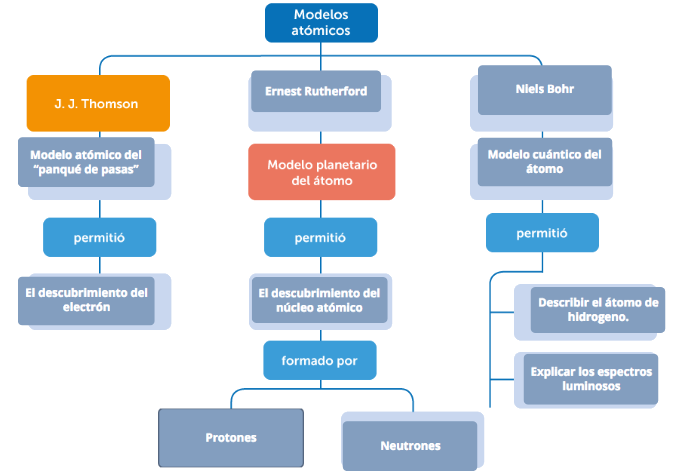
\includegraphics[width=\textwidth]{../images/SINFI_U2_AC65_IMGS1_sol.png}
              }\else{
                    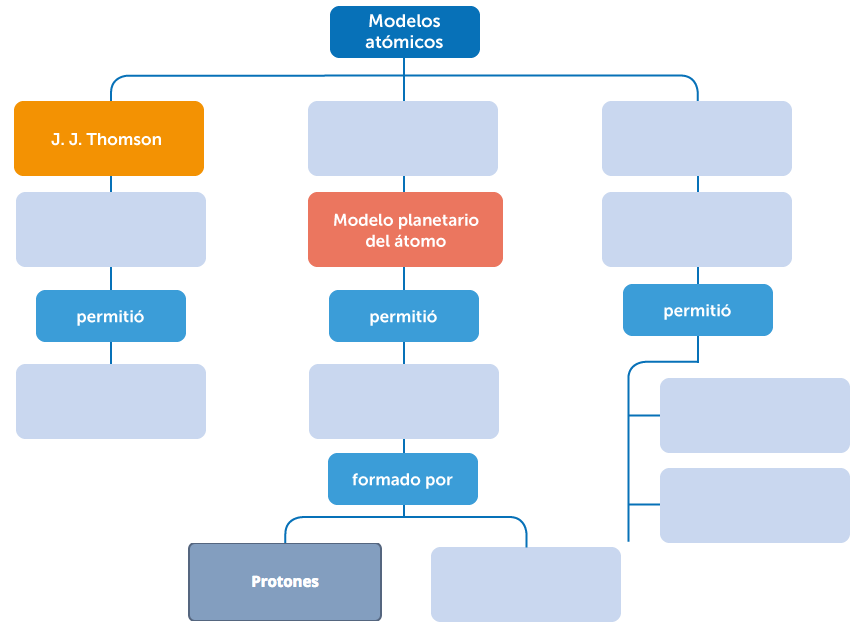
\includegraphics[width=\textwidth]{../images/SINFI_U2_AC65_IMGS1.png}
              }\fi          \end{minipage}
     }

\questionboxed[3]{Completa las oraciones sobre los modelos atómicos colocando la frase correcta:

 \begin{center}
              \wordpill{modelo atómico del ``panque de pasas''}
               \wordpill{el descubrimiento del electrón} 
              \wordpill{Ernest Rutherford}  
                \wordpill{el descubrimiento del núcleo atómico}
               \wordpill{neutrones}  
           \wordpill{Niels Bohr} 
              \wordpill{modelo cuántico del átomo}  
                \wordpill{describir el átomo de hidrógeno}
               \wordpill{explicar los espectros luminosos}  
          \end{center}
          \vspace*{1em}

\begin{parts}
    \part El modelo atómico de J.J. Thomson es conocido como el \fillin[modelo atómico del ``panque de pasas''] y permitió \fillin[el descubrimiento del electrón].
    
    \part El modelo atómico de \fillin[Ernest Rutherford] es el modelo planetario del átomo que permitió \fillin[el descubrimiento del núcleo atómico] formado por protones y \fillin[neutrones].
    
    \part El modelo atómico de \fillin[Niels Bohr] es conocido como el \fillin[modelo cuántico del átomo] y permitió \fillin[describir el átomo de hidrógeno] y \fillin[explicar los espectros luminosos].
\end{parts}
}

\questionboxed[2]{A partir de las siguientes descripciones visuales, identifica de qué modelo atómico se trata:

\begin{parts}
    \part Un esquema que muestra a un electrón saltando entre diferentes órbitas circulares concéntricas y absorbiendo o emitiendo energía en forma de luz:
  
    \begin{oneparchoices}
        \choice J.J. Thomson \choice Ernest Rutherford \CorrectChoice Niels Bohr
    \end{oneparchoices}
    
    \part Una esfera naranja continua de carga positiva que tiene incrustadas varias partículas pequeñas con carga negativa en su interior:
 
    \begin{oneparchoices}
        \CorrectChoice J.J. Thomson \choice Ernest Rutherford \choice Niels Bohr
    \end{oneparchoices}
\end{parts}
}
%      \questionboxed[5]{Clasifica cada uno de los siguientes elementos marcando con una \textbf{X} el grupo al que pertenece (si es materia o no es materia).

% \vspace{0.3cm}
% \begin{center}
% \renewcommand{\arraystretch}{1.3}
% \begin{tabularx}{0.8\textwidth}{l X c c}
% \toprule
% \textbf{No.} & \textbf{Elemento} & \textbf{Es materia} & \textbf{No es materia} \\
% \midrule
% 1 & La sal & ( \quad ) & ( \quad ) \\
% 2 & El color & ( \quad ) & ( \quad ) \\
% 3 & El agua & ( \quad ) & ( \quad ) \\
% 4 & El tiempo & ( \quad ) & ( \quad ) \\
% 5 & El papel & ( \quad ) & ( \quad ) \\
% 6 & El frío & ( \quad ) & ( \quad ) \\
% 7 & La miel & ( \quad ) & ( \quad ) \\
% 8 & El calor & ( \quad ) & ( \quad ) \\
% 9 & Una pluma & ( \quad ) & ( \quad ) \\
% 10 & Una idea & ( \quad ) & ( \quad ) \\
% 11 & Una silla & ( \quad ) & ( \quad ) \\
% 12 & La información & ( \quad ) & ( \quad ) \\
% \bottomrule
% \end{tabularx}
% \end{center}
%      }

\subsection{L10 La teoría atómica}

\ejemplosboxed[5]{Señala si son \textit{verdaderas} o \textit{falsas} las siguientes frases:

          \begin{multicols}{2}
               \begin{parts}\footnotesize%
                    \part Los electrones son partículas tan pequeñas que no es posible observarlas a simple vista, pero podemos saber de ellas a través de fenómenos como la electricidad, los espectros luminosos y el magnetismo.

                    \begin{oneparchoices}
                         \CorrectChoice Verdadero \choice Falso
                    \end{oneparchoices}

                    \part Los electrones son partículas de carga negativa cubiertas por una nube de carga positiva; la magnitud de ambas cargas es igual, por lo que son eléctricamente neutros.

                    \begin{oneparchoices}
                         \choice Verdadero \CorrectChoice Falso
                    \end{oneparchoices}

                    \part Todos los elementos radiactivos pueden emitir partículas llamadas alfa (carga positiva), beta (carga negativa) y gama (sin carga).

                    \begin{oneparchoices}
                         \CorrectChoice Verdadero \choice Falso
                    \end{oneparchoices}

                    \part En su experimento con partículas alfa, Rutherford encontró que algunas de éstas rebotaban después de chocar con la lámina metálica, por lo que concluyó que colisionaban con obstáculos de carga positiva.

                    \begin{oneparchoices}
                         \CorrectChoice Verdadero \choice Falso
                    \end{oneparchoices}

                    \part Todos los elementos emiten partículas alfa, que poseen carga positiva; beta, que tienen carga negativa; y rayos gama, que no tienen carga eléctrica.

                    \begin{oneparchoices}
                         \choice Verdadero \CorrectChoice Falso
                    \end{oneparchoices}

                    \columnbreak

                    \part El núcleo está formado por protones, que tienen carga positiva, y neutrones, que no poseen carga (es decir, son eléctricamente neutros).

                    \begin{oneparchoices}
                         \CorrectChoice Verdadero \choice Falso
                    \end{oneparchoices}

                    \part Cuando Rutherford colisionó partículas alfa sobre una lámina metálica delgada, encontró que se desviaban muy poco de su trayectoria original, por lo que de inmediato concluyó que el modelo atómico de Thomson era correcto.

                    \begin{oneparchoices}
                         \choice Verdadero \CorrectChoice Falso
                    \end{oneparchoices}

                    \part El modelo de Rutherford no pudo explicar por qué aparecían delgadas líneas oscuras entre las franjas de colores del espectro producido por la luz del Sol; este fenómeno sólo encontraría respuesta con el modelo atómico de Niels Bohr.


                    \begin{oneparchoices}
                         \CorrectChoice Verdadero \choice Falso
                    \end{oneparchoices}

                    \part Si los átomos estuvieran formados sólo por electrones, cualquier objeto estaría cargado negativamente y su electricidad sería evidente.

                    \begin{oneparchoices}
                         \CorrectChoice Verdadero \choice Falso
                    \end{oneparchoices}
               \end{parts}
          \end{multicols}

     }

     \questionboxed[3]{Indica si cada afirmación sobre los modelos atómicos es Verdadera (V) o Falsa (F).

\begin{parts}
    \part \underline{\hspace{1cm}} Cuando Rutherford colisionó partículas alfa sobre una lámina metálica delgada, concluyó de inmediato que el modelo atómico de Thomson era correcto.
    \part \underline{\hspace{1cm}} El modelo de Rutherford no pudo explicar por qué aparecían delgadas líneas oscuras en el espectro producido por la luz solar; este fenómeno sólo encontraría respuesta con Niels Bohr.
    \part \underline{\hspace{1cm}} El núcleo del átomo está formado por protones, que tienen carga positiva, y neutrones, que no poseen carga (son eléctricamente neutros).
    \part \underline{\hspace{1cm}} Si los átomos estuvieran formados sólo por electrones, cualquier objeto estaría cargado negativamente y su electricidad sería evidente.
    \part \underline{\hspace{1cm}} Los electrones son partículas tan pequeñas que no es posible observarlos a simple vista, pero podemos saber de ellos a través de fenómenos como la electricidad y el magnetismo.
    \part \underline{\hspace{1cm}} La clásica figura de un núcleo central con múltiples electrones orbitando en trayectorias elípticas entrelazadas es una representación del modelo atómico original de Thomson.
\end{parts}
     }

\questionboxed[3]{Relaciona la aportación científica o característica con el modelo o científico al que pertenece, escribiendo la letra correspondiente en el paréntesis. Algunas opciones pueden repetirse o sobrar.

\vspace{0.3cm}
\begin{minipage}[t]{0.75\textwidth}
    \begin{itemize}
        \item[(\quad)] Demostró que los rayos catódicos son partículas cargadas negativamente y provienen de los átomos.
        \item[(\quad)] Concibió un modelo conocido como ``panqué de pasas''.
        \item[(\quad)] Demostró que la carga positiva no era una especie de nube, sino un núcleo.
        \item[(\quad)] Aseguró que los electrones sólo giran en órbitas determinadas alrededor del núcleo.
        \item[(\quad)] Explicó la existencia de líneas oscuras en el espectro luminoso del hidrógeno por el intercambio de energía.
        \item[(\quad)] Concibió un modelo atómico planetario en el que el Sol representaba al núcleo y los planetas a los electrones.
        \item[(\quad)] Explicó que los electrones desprenden una cantidad fija de energía (luz) al regresar a órbitas menos energéticas.
        \item[(\quad)] Calculó los radios de las órbitas en las cuales un electrón podría girar alrededor del núcleo.
        \item[(\quad)] Demostró que el plutonio, el uranio, el radio y el polonio son elementos radiactivos.
    \end{itemize}
\end{minipage}
\hfill
\begin{minipage}[t]{0.2\textwidth}
    \begin{itemize}
        \item[A.] J. J. Thomson
        \item[B.] E. Rutherford
        \item[C.] Niels Bohr
        \item[D.] Ninguno
    \end{itemize}
\end{minipage}
}

% \questionboxed[5]{Indica a qué científico pertenece cada aportación (J.J. Thomson, Ernest Rutherford, Niels Bohr, o Ninguno):
% \begin{parts}
%     \part Demostró que los rayos catódicos son partículas cargadas negativamente y que provienen de los átomos de la materia. (\textbf{J.J. Thomson})
%     \part Concibió un modelo de átomo conocido como ``panqué de pasas'' donde el pan representaba la carga positiva y las ``pasas'', las cargas negativas. (\textbf{J.J. Thomson})
%     \part Con base en sus experimentos con materiales radiactivos, demostró que la carga positiva no era una especie de nube que envuelve a los electrones. (\textbf{Ernest Rutherford})
%     \part Aceptando parcialmente el modelo de Rutherford, aseguró que los electrones sólo giran en órbitas determinadas alrededor del núcleo. (\textbf{Niels Bohr})
%     \part Formuló un modelo que permitió explicar la existencia de líneas oscuras en el espectro luminoso del hidrógeno, y demostró que éstas tenían su origen en el intercambio de energía con los electrones en el núcleo. (\textbf{Niels Bohr})
%     \part Concibió un modelo atómico planetario en el que el Sol representaba al núcleo y los planetas representaban los electrones que orbitaban alrededor de éste. (\textbf{Ernest Rutherford})
%     \part Explicó que, cuando regresan a órbitas menos energéticas, los electrones deben desprenderse de una cantidad fija de energía y que ésta se manifiesta como luz. (\textbf{Niels Bohr})
%     \part Aseguró que en la naturaleza la energía no es continua, sino que se presenta en múltiplos de una cantidad fija conocida como cuanto. (\textbf{Niels Bohr})
%     \part Demostró que el plutonio, el uranio, el radio y el polonio son elementos radiactivos, pues emitían partículas alfa, beta y gama. (\textbf{Ninguno})
% \end{parts}
% }



\subsection{L11 Estados de agregación de la materia y modelo cinético}

\ejemplosboxed[5]{Coloca los conceptos en el lugar que les corresponda en la imagen.

          \begin{minipage}[t][][b]{.55\textwidth}\Large
               \wordpill{Sublimación} \wordpill{Fusión} \wordpill{Ebullición} \wordpill{Gaseoso} \wordpill{Sólido} \wordpill{Solidificación} \wordpill{Deposición} \wordpill{Líquido} \wordpill{Condensación}
          \end{minipage}\hfill%
          \begin{minipage}[t][][b]{.4\textwidth}
               \ifprintanswers{
                    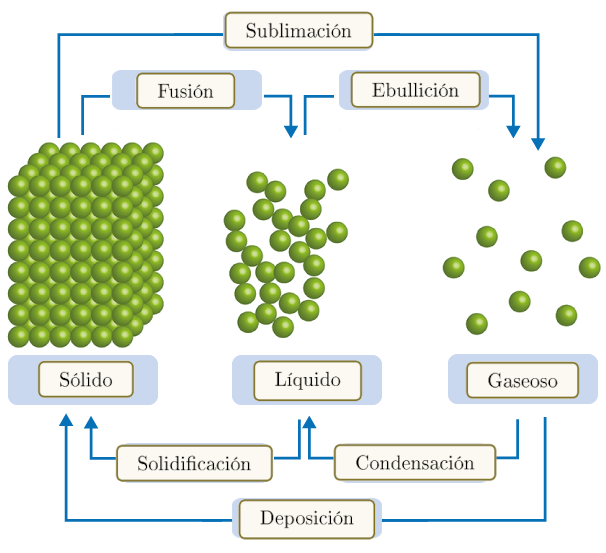
\includegraphics[width=\linewidth]{../images/SINFI_U2_AC47_IMG1_SOL.png}
               }\else{
                    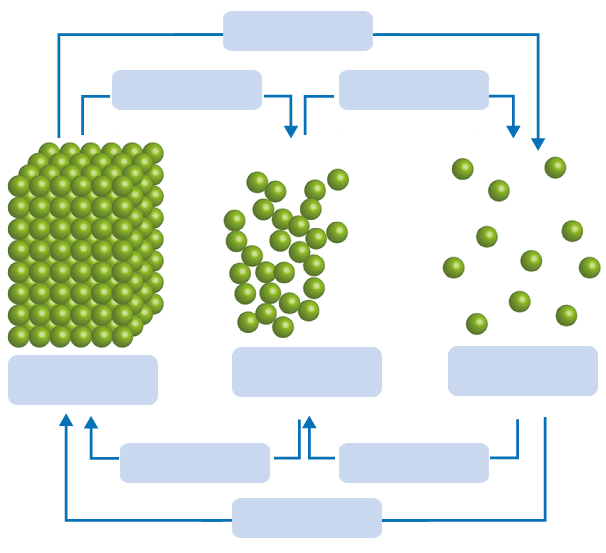
\includegraphics[width=\linewidth]{../images/SINFI_U2_AC47_IMG1.png}
               }\fi
          \end{minipage}
     }

\questionboxed[2]{Identifica a qué estado de la materia (\textbf{Sólido, Líquido o Gaseoso}) hace referencia cada descripción.

\begin{parts}
    \part \underline{\hspace{3cm}} ¿Qué estado de agregación se caracteriza por el hecho de que las partículas están muy próximas entre sí y su único movimiento es el de vibración?
    
    \vspace{0.3cm}
    \part \underline{\hspace{3cm}} Si un cuerpo de $1\text{ m}^3$ adopta la forma del recipiente que lo contiene, considerando que no cambia su volumen, ¿en qué estado de agregación se encuentra?
    
    \vspace{0.3cm}
    \part \underline{\hspace{3cm}} Un cuerpo fluye por una tubería y cambia de volumen cuando ingresa a un depósito más grande. ¿De qué estado de agregación se trata?
    
    \vspace{0.3cm}
    \part \underline{\hspace{3cm}} Un cuerpo que se encontraba en un recipiente cambió de densidad al trasladarse a otro tres veces más pequeño. ¿Cuál es su estado de agregación?
\end{parts}
}


     \subsection{L12 Temperatura y equilibrio térmico}

 \ejemplosboxed[10]{Elige la respuesta para cada pregunta.
          \begin{multicols}{2}
               \begin{parts}
                    \part Un corresponsal de noticias informa que las altas temperaturas en California, Estados Unidos, alcanzaron 113 °F. ¿Cuál es la temperatura equivalente en grados centígrados?

                    \begin{oneparchoices}
                         \CorrectChoice 45 °C \choice 55 °C
                    \end{oneparchoices}

                    % \part José observa el informe del clima durante un viaje de negocios en Dublín (Irlanda). El conductor de noticias asegura que la temperatura se elevará de los 64.4 °F actuales a 102.2 °F. ¿Cuál es el incremento de temperatura correspondiente en la escala Celsius?

                    % \begin{oneparchoices}
                    %      \CorrectChoice 21 °C \choice 37.8 °C
                    % \end{oneparchoices}

 \part El punto de fusión del oro es 1 064 °C y la plata se funde a 1 234.93 K. ¿Cuál de los dos tiene una temperatura de fusión más elevada?

                    \begin{oneparchoices}
                         \CorrectChoice El oro \choice La plata
                    \end{oneparchoices}

                    \part Pedro se siente mal y decide ir al médico, éste le informa que su temperatura corporal es de 313.15 K. Pedro sabe que una persona tiene fiebre cuando su temperatura es superior a 37 °C. ¿Cuál es el estado de salud de Pedro?

                    \begin{choices}
                          \choice Pedro no tiene fiebre
                          \CorrectChoice Pedro tiene fiebre
                    \end{choices}

                    % \part Mónica cocinará un pavo en Navidad y desea que su familia realmente lo disfrute, por lo que se prepara estudiando un recetario de cocina profesional. En él encuentra que debe precalentar el horno a 325 °F, pero su horno utiliza la escala Celsius. ¿Cuál es la temperatura equivalente?

                    % \begin{oneparchoices}
                    %      \CorrectChoice 100 °C \choice 162.7 °C
                    % \end{oneparchoices}

                    \part De compras en un centro comercial, Francisco lee en la etiqueta de una lata de atún: “Mantener por debajo de 296.15 K. ¿Cuál es la temperatura correspondiente en la escala Celsius?

                    \begin{oneparchoices}
                         \CorrectChoice 23 °C \choice 47 °C
                    \end{oneparchoices}


                    \part Mexicali, capital de Baja California, es la ciudad más calurosa de México. Debido a su ubicación de tipo desierto interior, las temperaturas alcanzan 40 °C. ¿A qué temperatura equivale esto en la escala Fahrenheit?

                    \begin{oneparchoices}
                         \CorrectChoice 72 °F \choice 104 °F
                    \end{oneparchoices}

                    % \part El cuerpo humano resiste mejor los descensos de temperatura que los aumentos en la misma. Un descenso significativo de temperatura sólo provoca una lentificación de las funciones celulares, mientras que un aumento de la misma magnitud provocaría la pérdida definitiva de tales funciones. La temperatura máxima que puede soportar el cuerpo humano es 316.15 K. ¿A qué temperatura equivale en la escala Celsius y Fahrenheit?

                    % \begin{oneparchoices}
                    %      \choice 109,4 °C y 43 °F \CorrectChoice 43 °C y 109.4 °F
                    % \end{oneparchoices}

                    \part El 10 de agosto del 2010, un grupo de investigadores registró en la Antártida la temperatura más baja del planeta: 93 °C bajo cero. ¿Cuál es la temperatura correspondiente en la escala de temperatura absoluta?

                    \begin{oneparchoices}
                         \CorrectChoice 180.15 K \choice 366.15 K
                    \end{oneparchoices}

                    % \part Venus no es el planeta más cercano al Sol, pero sí el más caliente, pues posee una atmósfera muy densa que impide que el calor proveniente del Sol escape del planeta (efecto invernadero). Alcanza temperaturas de hasta 864 °F. ¿Cuál es la temperatura correspondiente en la escala Celsius?

                    % \begin{oneparchoices}
                    %      \CorrectChoice 462.22 °C \choice 1587.2 °C
                    % \end{oneparchoices}

                    % \part Rubén colocó un vaso con agua en el refrigerador y lo dejó ahí hasta que el agua sufrió un descenso de temperatura de 20.3 °C. ¿Cuál es el cambio de temperatura correspondiente en K?

                    % \begin{oneparchoices}
                    %      \choice 20.3 K \CorrectChoice 293.45 K
                    % \end{oneparchoices}

                    % \part Según la agencia científica de Naciones Unidas, la temperatura promedio en la superficie de la Tierra y de los océanos fue la más alta en el periodo de enero a octubre de 2014, al alcanzar 14.78 °C. ¿Cuál es la temperatura correspondiente en grados Fahrenheit?

                    % \begin{oneparchoices}
                    %      \choice 26.604 °F \CorrectChoice  58.604 °F
                    % \end{oneparchoices}

                   

               \end{parts}
          \end{multicols}

     }

     \questionboxed[3]{Lee cada situación y elige la respuesta correcta para cada pregunta:

     \begin{parts}
    \part Un corresponsal de noticias informa que las altas temperaturas en California, Estados Unidos, alcanzaron $113 \ ^\circ\text{F}$. ¿Cuál es la temperatura equivalente en grados centígrados?
   
    \begin{oneparchoices}
        \CorrectChoice $45 \ ^\circ\text{C}$ \choice $55 \ ^\circ\text{C}$
    \end{oneparchoices}

    \part José observa el informe del clima durante un viaje de negocios en Dublín (Irlanda). El conductor de noticias asegura que la temperatura se elevará de los $64.4 \ ^\circ\text{F}$ actuales a $102.2 \ ^\circ\text{F}$. ¿Cuál es el incremento de temperatura correspondiente en la escala Celsius?
  
    \begin{oneparchoices}
        \CorrectChoice $21 \ ^\circ\text{C}$ \choice $37.8 \ ^\circ\text{C}$
    \end{oneparchoices}

    \part Pedro se siente mal y decide ir al médico. Éste le informa que su temperatura corporal es de $313.15 \text{ K}$. Pedro sabe que una persona tiene fiebre cuando su temperatura es superior a $37 \ ^\circ\text{C}$. ¿Cuál es su estado de salud?
  
    \begin{oneparchoices}
        \CorrectChoice Pedro tiene fiebre \choice Pedro no tiene fiebre
    \end{oneparchoices}

    \part Mónica cocinará un pavo en Navidad y desea que su familia realmente lo disfrute, por lo que se prepara estudiando un recetario de cocina profesional. En él encuentra que debe precalentar el horno a $325 \ ^\circ\text{F}$, pero su horno utiliza la escala Celsius. ¿Cuál es la temperatura equivalente?
 
    \begin{oneparchoices}
        \choice $100 \ ^\circ\text{C}$ \CorrectChoice $162.7 \ ^\circ\text{C}$
    \end{oneparchoices}

    \part De compras en un centro comercial, Francisco lee en la etiqueta de una lata de atún: ``Mantener por debajo de $296.15 \text{ K}$''. ¿Cuál es la temperatura correspondiente en la escala Celsius?

    \begin{oneparchoices}
        \CorrectChoice $23 \ ^\circ\text{C}$ \choice $47 \ ^\circ\text{C}$
    \end{oneparchoices}

    \part Mexicali, capital de Baja California, es la ciudad más calurosa de México. Debido a su ubicación de tipo desierto interior, las temperaturas alcanzan $40 \ ^\circ\text{C}$. ¿A qué temperatura equivale esto en la escala Fahrenheit?
  
    \begin{oneparchoices}
        \choice $72 \ ^\circ\text{F}$ \CorrectChoice $104 \ ^\circ\text{F}$
    \end{oneparchoices}

    \part La temperatura máxima que puede soportar el cuerpo humano es $316.15 \text{ K}$. ¿A qué temperatura equivale en las escalas Celsius y Fahrenheit?
  
    \begin{oneparchoices}
        \choice $109.4 \ ^\circ\text{C}$ y $43 \ ^\circ\text{F}$ \CorrectChoice $43 \ ^\circ\text{C}$ y $109.4 \ ^\circ\text{F}$
    \end{oneparchoices}

    \part El 10 de agosto del 2010, un grupo de investigadores registró en la Antártida la temperatura más baja del planeta: $93 \ ^\circ\text{C}$ bajo cero. ¿Cuál es la temperatura correspondiente en la escala de temperatura absoluta?
 
    \begin{oneparchoices}
        \CorrectChoice $180.15 \text{ K}$ \choice $366.15 \text{ K}$
    \end{oneparchoices}

    \part Venus alcanza temperaturas de hasta $864 \ ^\circ\text{F}$. ¿Cuál es la temperatura correspondiente en la escala Celsius?
    
    \begin{oneparchoices}
        \CorrectChoice $462.22 \ ^\circ\text{C}$ \choice $1587.2 \ ^\circ\text{C}$
    \end{oneparchoices}

    \part Rubén colocó un vaso con agua en el refrigerador y lo dejó ahí hasta que el agua sufrió un descenso de temperatura de $20.3 \ ^\circ\text{C}$. ¿Cuál es el cambio de temperatura correspondiente en K?
   
    \begin{oneparchoices}
        \choice $20.3 \text{ K}$ \CorrectChoice $293.45 \text{ K}$ % Nota: Marcada así en la imagen original
    \end{oneparchoices}

    \part La temperatura promedio en la superficie de la Tierra y océanos alcanzó $14.78 \ ^\circ\text{C}$ en 2014. ¿Cuál es la temperatura correspondiente en grados Fahrenheit?
   
    \begin{oneparchoices}
        \choice $26.604 \ ^\circ\text{F}$ \CorrectChoice $58.604 \ ^\circ\text{F}$
    \end{oneparchoices}

    \part El punto de fusión del oro es $1064 \ ^\circ\text{C}$ y la plata se funde a $1234.93 \text{ K}$. ¿Cuál de los dos tiene una temperatura de fusión más elevada?
  
    \begin{oneparchoices}
        \CorrectChoice El oro \choice La plata
    \end{oneparchoices}
\end{parts}
     }